\section{Experimental Results and Discussion}

%%%% BECHMARKS
\begin{table*}[t]
\begin{center}
\begin{small}
\begin{tabular}{llll}
\hline
\textbf{Task}  & \textbf{Benchmark} & \textbf{\textit{in-domain} Test set} & \textbf{\textit{out-of-domain} Test set} \\ \hline
\pos (\accuracy)    & \best{0.972} \cite{Toutanova:2003} & 0.959 (\Skipgram[\withup]) & 0.910 (\Skipgram)\\ 
\chunking (\fscore) & \best{0.942} \cite{Sha:2003} & 0.938 (\brown[b = 2000]) & 0.676 (\Glove)\\  
\ner (\fscore)      & \best{0.893} \cite{Ando:2005} & 0.868 (\Skipgram) & 0.736 (\Skipgram) \\  
\mwe (\fscore)      &0.625 \cite{Schneider+:2014} & \best{0.654} (\CW) & --- \\ %
\hline
\end{tabular}
\caption{State-of-the-art results vs.\ our best results for in-domain and
  out-of-domain test sets.}
\label{benchmark}
\end{small}
\end{center}
\end{table*}


%%%%%%%%%%%%%%%%%%%%%%%%%%%%
%%% HEATMAPS 
\begin{figure*}[t!]
\centering
\begin{subfigure}{7cm}
	\centering
    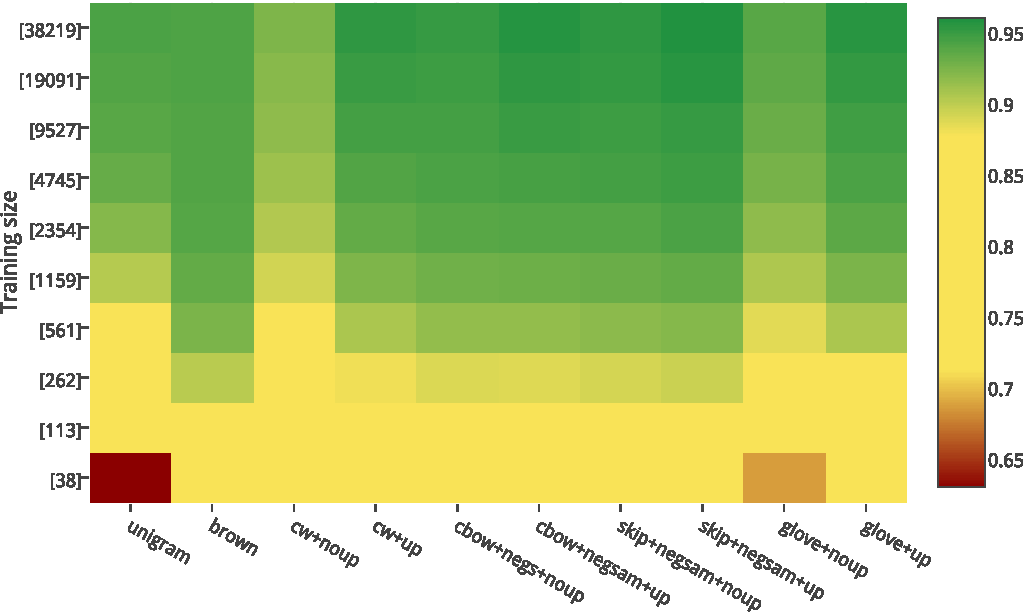
\includegraphics[scale=0.4]{plots/map-pos-color-invert}    	
	\subcaption{\pos (\accuracy)}	
	\label{pos}
\end{subfigure}
\begin{subfigure}{7cm}
	\centering
    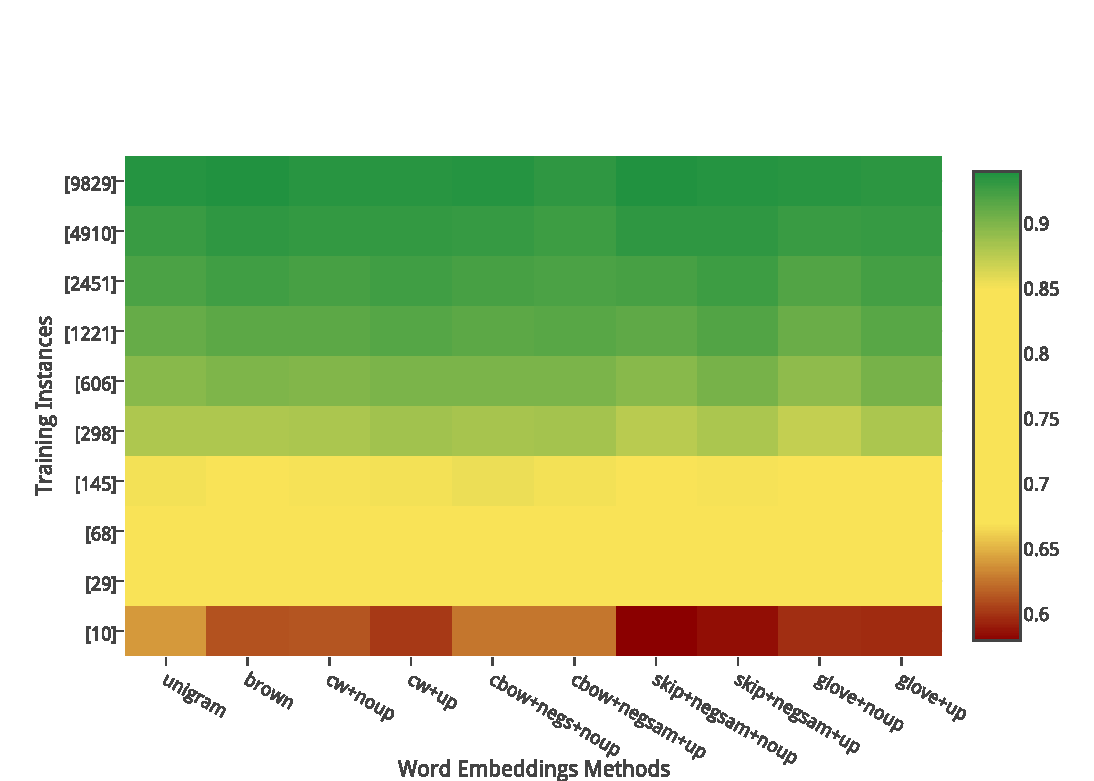
\includegraphics[scale=0.4]{plots/map-chunk-color-invert}
	\subcaption{\chunking (\fscore)}	
	\label{chu}
\end{subfigure}
%\\[-1.5ex]  %%<-- in this line
\begin{subfigure}{7cm}
	\centering
    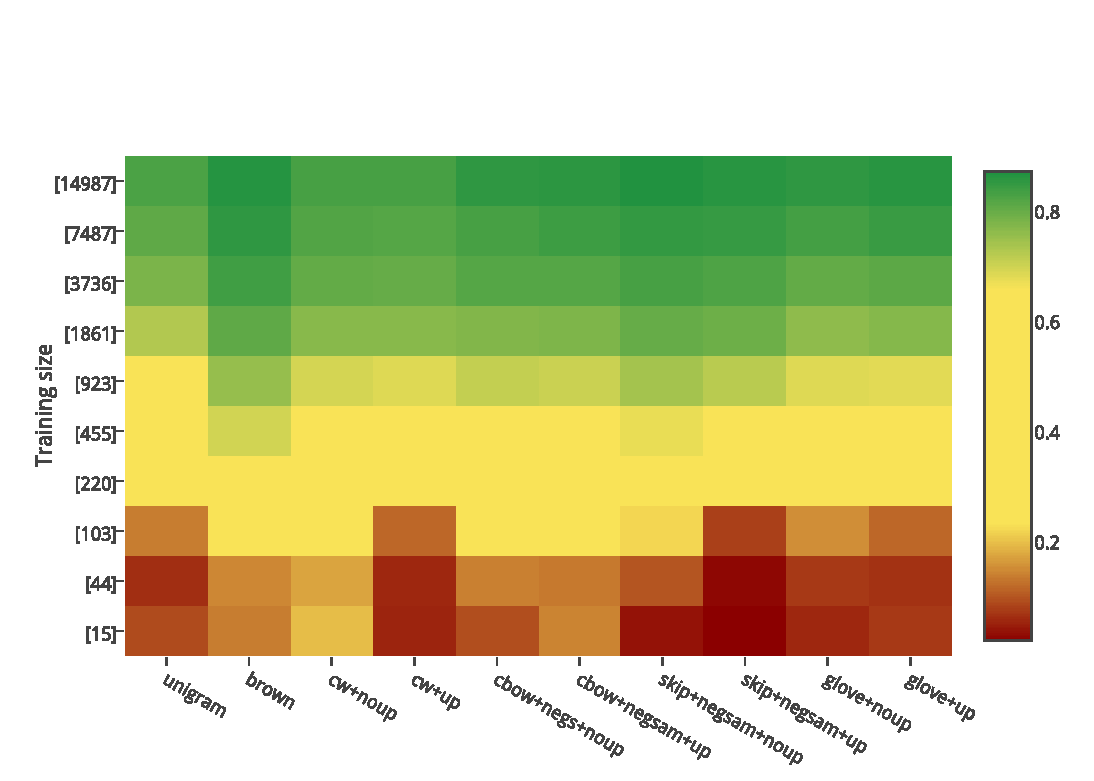
\includegraphics[scale=0.4]{plots/map-ner-color-invert}    	
	\subcaption{\ner (\fscore)}	
	\label{ner}
\end{subfigure}
\begin{subfigure}{7cm}
	\centering
    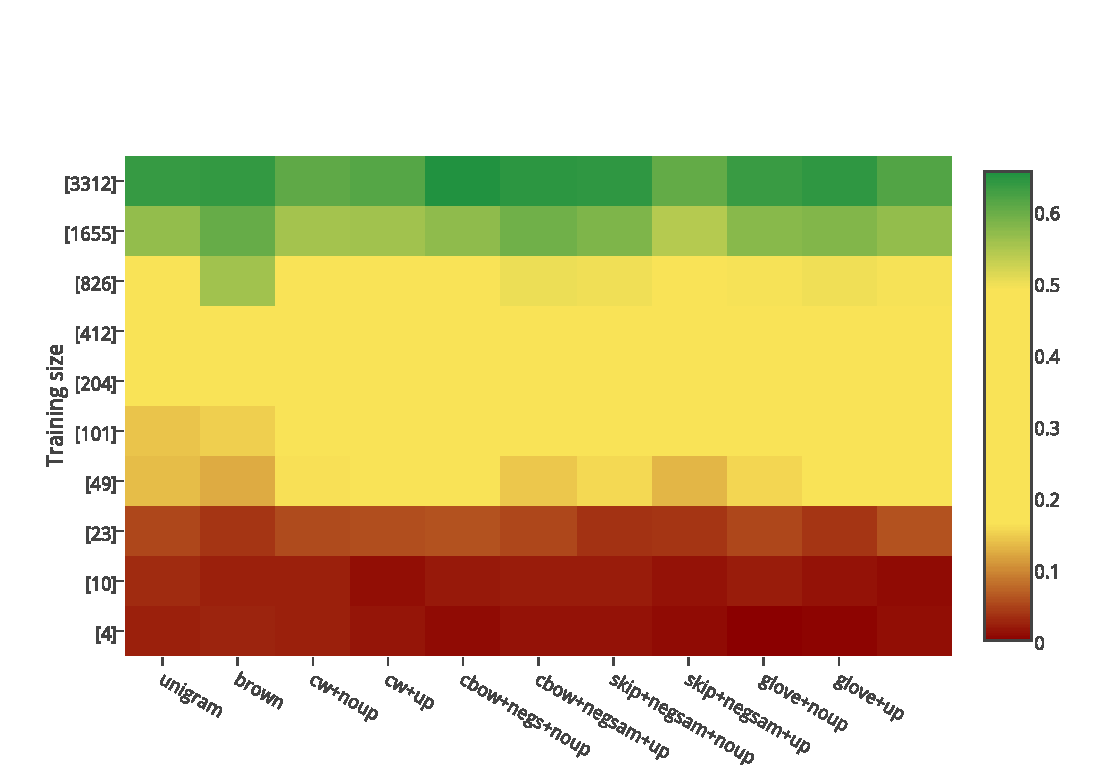
\includegraphics[scale=0.4]{plots/map-mwe-color-invert}
	\subcaption{\mwe (\fscore)}		
	\label{mwe}
\end{subfigure}
\caption{Results for each type of word representation over \pos, \chunking, \ner and
  \mwe, optionally with updating (``\withup''). The $y$-axis indicates the training data
  sizes (on a log scale). Green = high performance, and red = low
  performance, based on a linear scale of the best- to worst-result for
  each task. }
\label{fig:heatmaps}
\end{figure*}

%%%%%%%%%%%%%%%%%%%%%%%%%%%%
%%% OOV 
\begin{figure*}[t!]
\centering
    	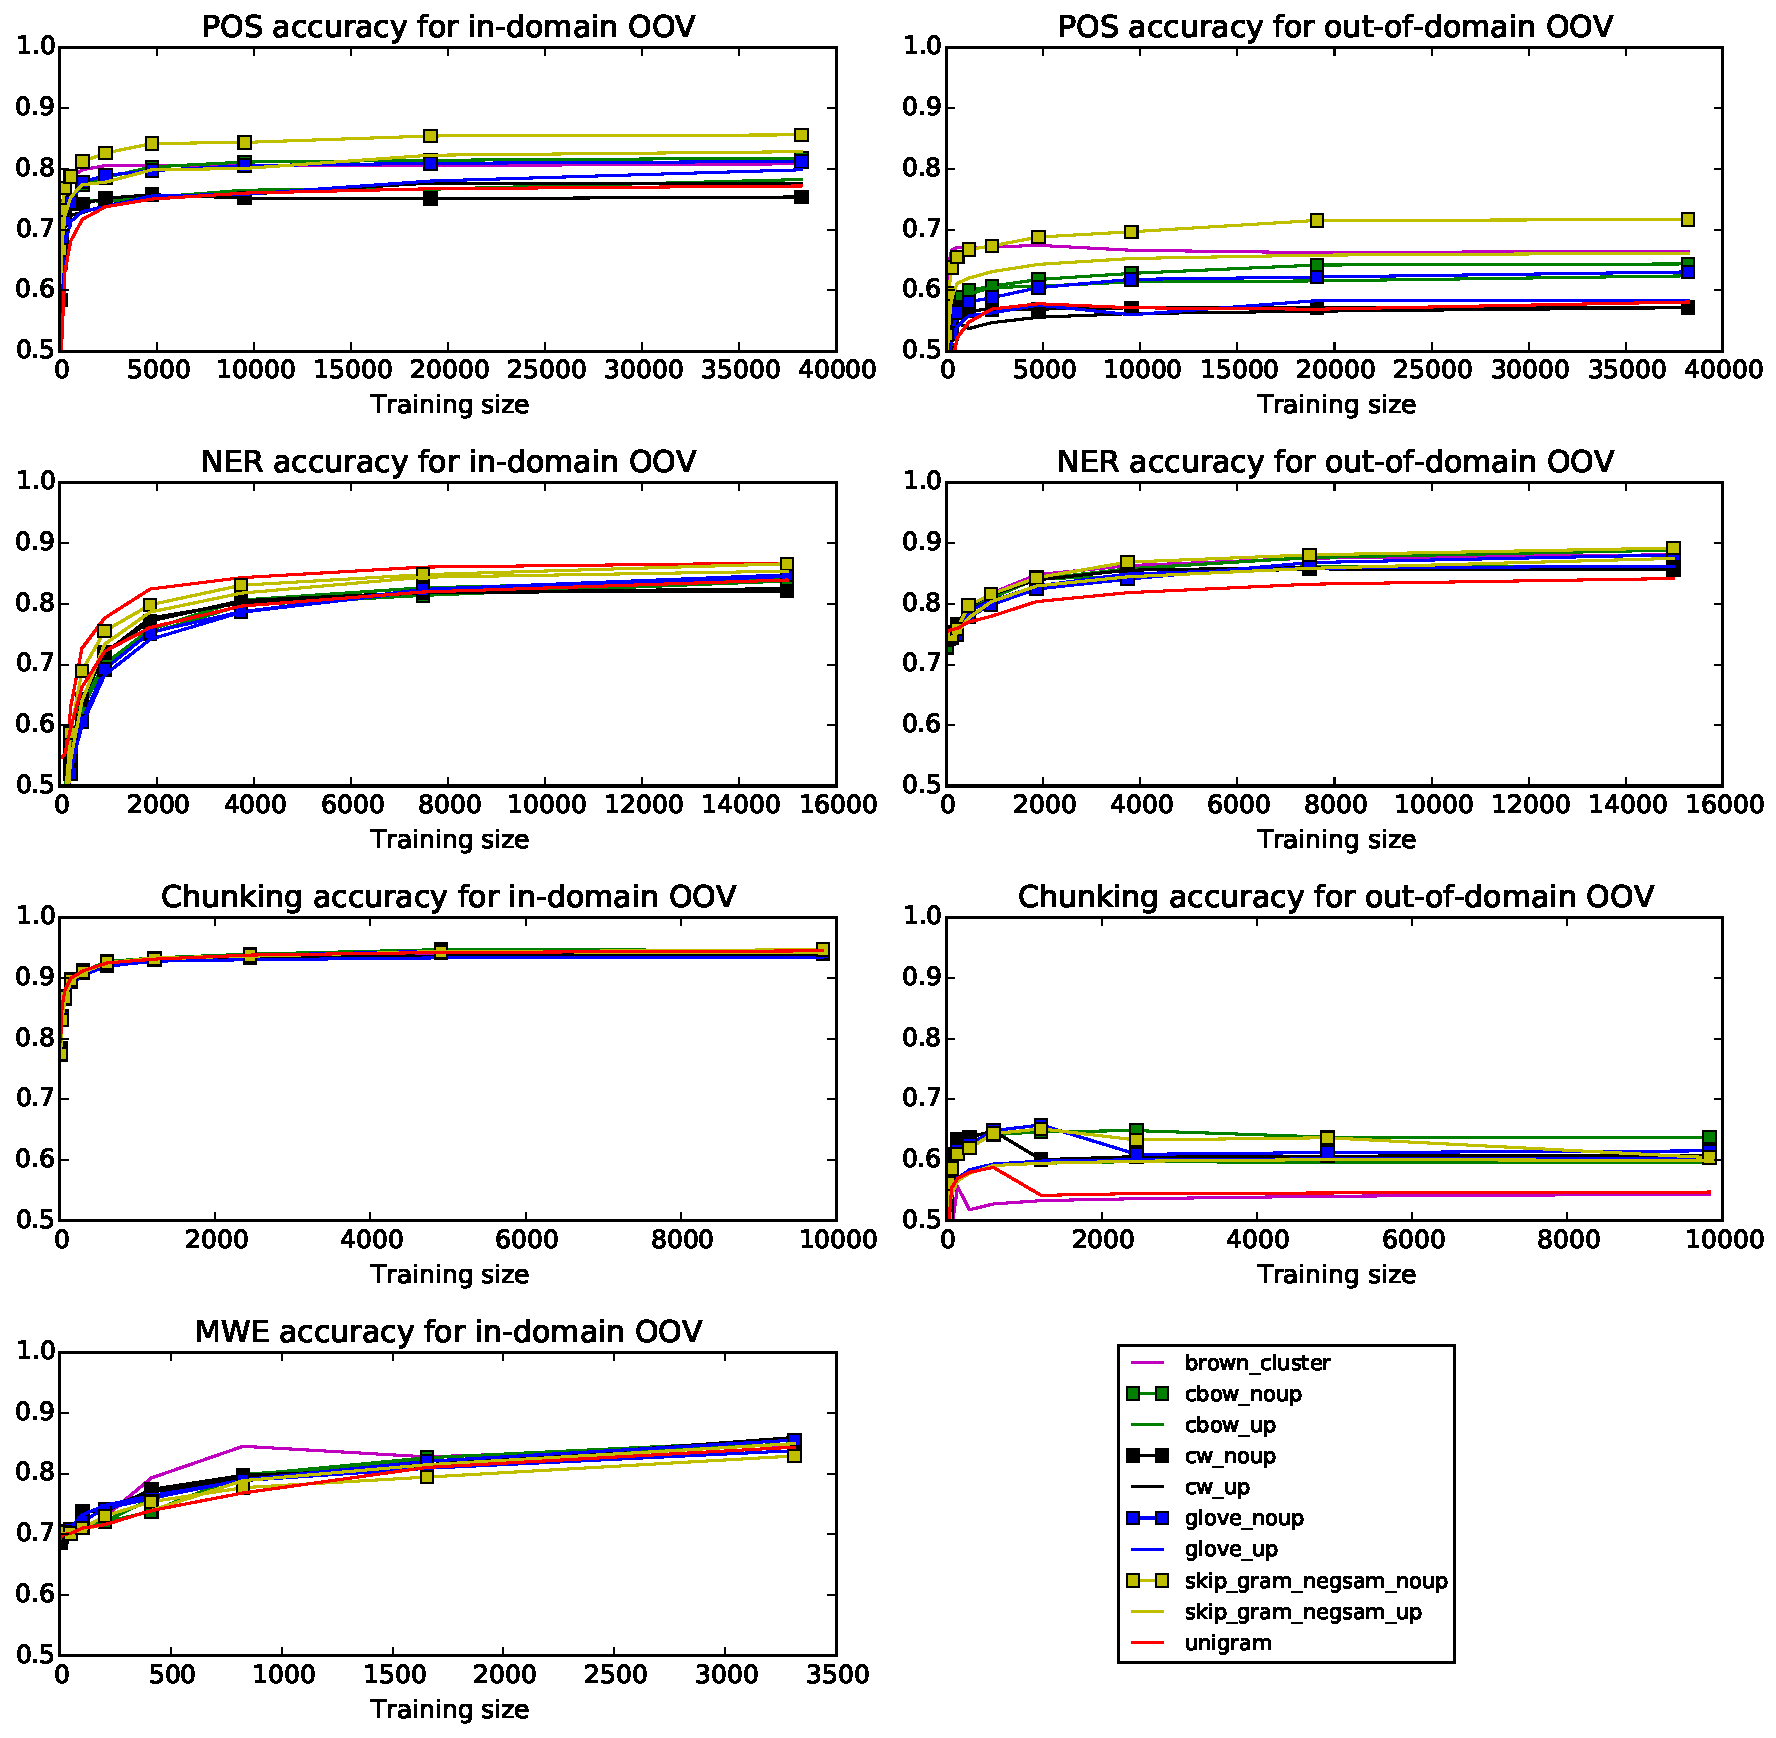
\includegraphics[scale=0.5]{plots/OOV-plots}
\caption{\accuracy over out-of-vocabulary (OOV) words for \textit{in-domain} and \textit{out-of-domain} test sets.}
\label{OOV} 
\end{figure*}



We structure our evaluation by stepping through each of our five
research questions (\RQ[1--5]) from the start of the paper. In this, we
make reference to: (1) the best-performing method both in- and
out-of-domain vs.\ the state-of-the-art (\tabref{benchmark}); (2) a
heat map for each task indicating the convergence rate for each word
representation, with and without updating (\figref{fig:heatmaps}); 
(3) OOV accuracy both in-domain and out-of-domain for each task
(\figref{OOV}); and (4)  visualization of the impact of
updating on word embeddings, based on t-SNE
(\figref{fig:vectorfield}).

%\textbf{(i) Are the evaluated word embedding methods better than unigram features?}
\paragraph{\RQ[1]: Are word embeddings better than one-hot unigram features
  and Brown clusters?}  As shown in \tabref{benchmark}, the
best-performing method for every task except in-domain \chunking is a
word embedding method, although the precise method varies
greatly. \figref{fig:heatmaps}, on the other hand, tells a more subtle
story: the difference between \unigram and the other word
representations is relatively modest, esp.\ as the amount of training
data increases. Additionally, the difference between \brown and the word
embedding methods is modest across all tasks. So, the overall answer
would appear to be: yes for unigrams when there is little training data, but not really for \brown.




%\textbf{(ii) How does the size of labelled training data affect the experimental results?}
\paragraph{\RQ[2]: Do word embedding features require less training data?}
\figref{fig:heatmaps} shows that for \pos and \ner, with only several hundred training instances, 
word embedding features achieve superior results to \unigram. 
For example, when trained with 561 instances, the \pos model using \Skipgram[\withup] embeddings is 5.3\% above
\unigram; and when trained with 932 instances, the \ner model using \Skipgram is 11.7\% above \unigram. 
Similar improvements are also found for other types of word embeddings and \brown, when the training set is small. 
However, all word representations perform similarly for \chunking
regardless of training data size.
For \mwe, \brown performs slightly better than the other methods when
trained with approximately 25\% of the training instances. 
Therefore, we conjecture that the \pos and \ner tasks benefit more from
distributional similarity than \chunking and \mwe.

\paragraph{\RQ[3]: Does task-specific updating improve all word embeddings across all tasks?}
Based on \figref{fig:heatmaps}, updating of word representations can
equally correct poorly-learned word representations, and harm
pre-trained representations, due to overfitting.
For example, \CW and \Glove perform significantly worse than \Skipgram
in both \pos and \ner without updating, but \emph{with} updating, the
gap between their results and the best performing method becomes
smaller. In contrast, \Skipgram performs worse over the test data with
updating, despite the results on the development set improving by 1\%.

To further investigate the effects of updating, we sampled 60 words and
plotted the changes in their word embeddings under updating, using 2-d
vector fields generated with t-SNE \cite{vanderMaaten:Hinton:2008}. Half
of the words were chosen manually to include known word clusters such as
days of the week and names of countries; the other half were selected
randomly. Additional plots with 100 randomly-sampled words and the
top-100 most frequent words, for all the methods and all the tasks, can
be found in the supplementary material and at
\url{https://123abc123abd.wordpress.com/}.  In each plot, a single arrow
signifies one word, pointing from the position of the original word embedding to the updated representation.

In \figref{fig:vectorfield}, we show vector fields plots for \chunking and \ner using \Skipgram embeddings.
For \chunking, most of the vectors were changed with similar magnitude,
but in very different directions, including within the clusters of days of
the week and country names.
In contrast, for \ner, there was more homogeneous change in word vectors
belonging to the same cluster.
This greater consistency is further evidence that semantic homogeneity
appears to be more beneficial for \ner than \chunking. 


%%%%%%%%%%%%%%%%%%%%%%%%%%%%
%%% Vector fields
% POS
\begin{figure*}[t!]
\centering
\begin{subfigure}[b]{0.48\textwidth}
	\centering
    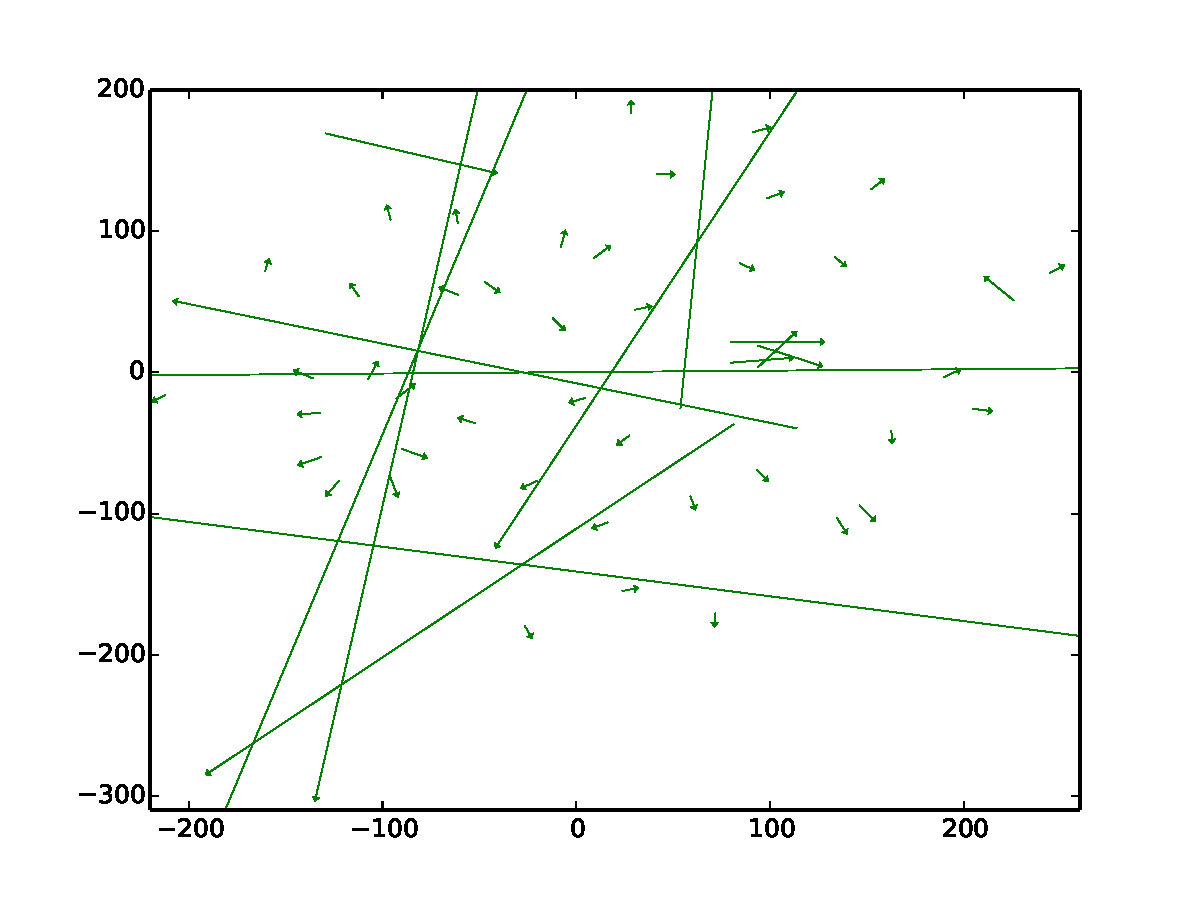
\includegraphics[width=\textwidth]{plots/vectorField/Lizhen/scaled/Lizhen_skip_chunking}
	\subcaption{\chunking}	
	\label{fig:skipChu}
\end{subfigure}
\begin{subfigure}[b]{0.48\textwidth}
	\centering
    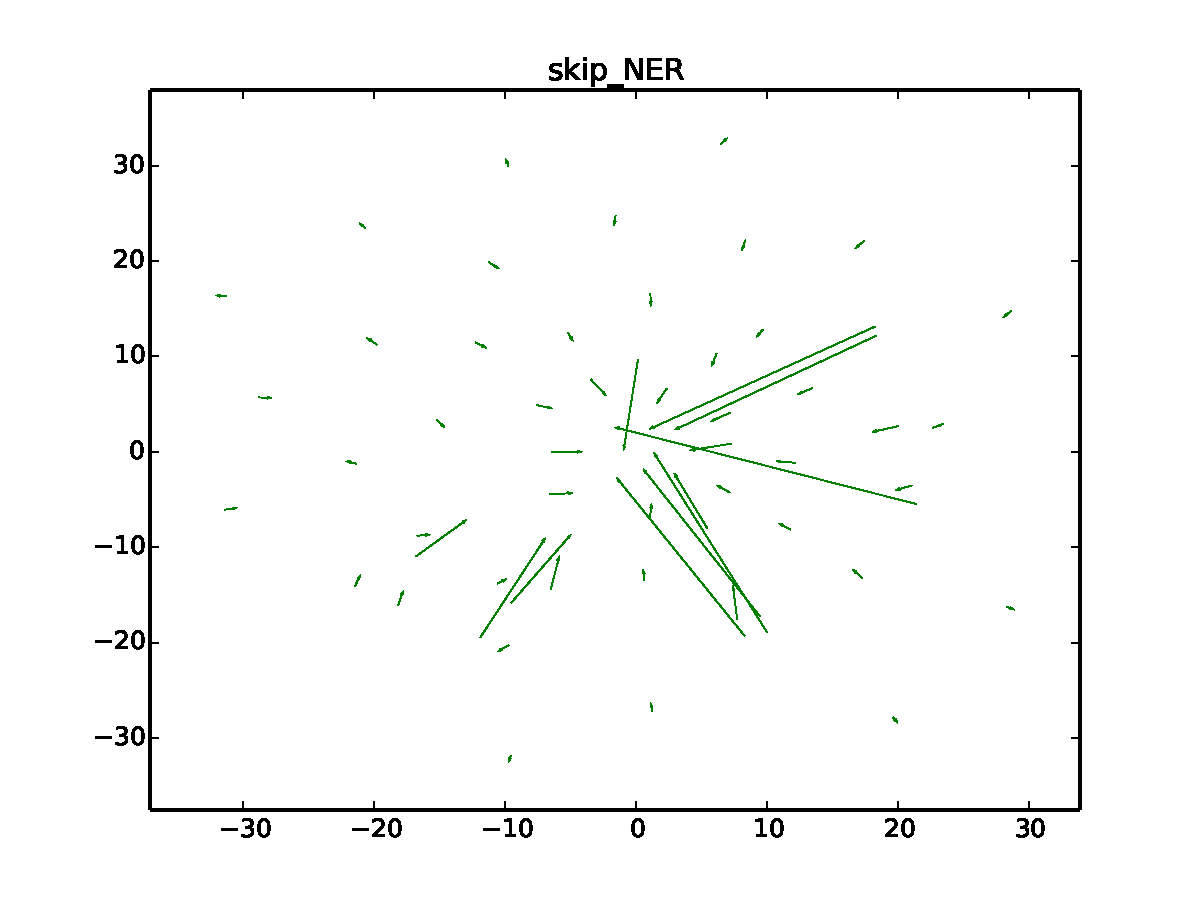
\includegraphics[width=\textwidth]{plots/vectorField/Lizhen/Lizhen_skip_NER}    	
	\subcaption{\ner}
	\label{fig:skippos}	
\end{subfigure}
%\begin{subfigure}[b]{0.48\textwidth}
%	\centering
%   \includegraphics[width=\textwidth]{plots/vectorField/skip_\ner.png}
%	\label{fig:skipner}
%	\subcaption{}	
%\end{subfigure}
%%\begin{subfigure}{6cm}
%	\centering
 %   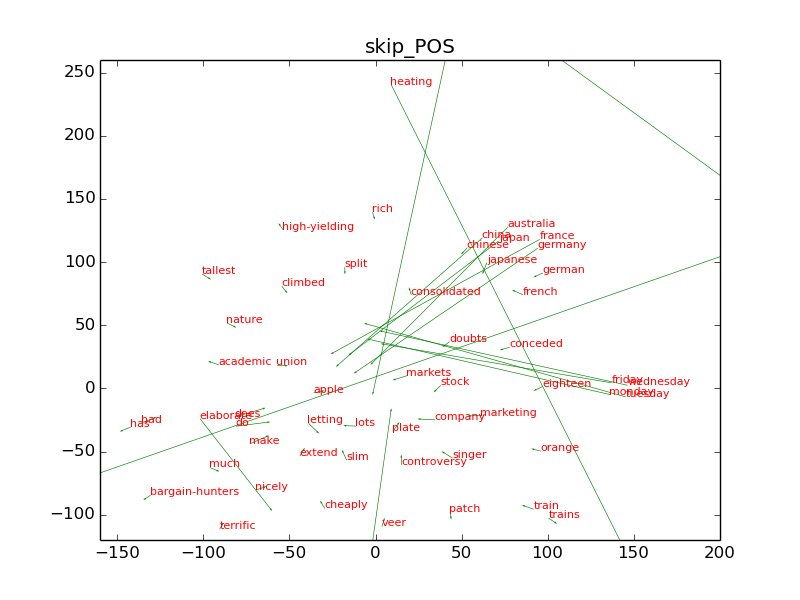
\includegraphics[scale=0.3]{plots/vectorField/skip_POS.png}
%	\label{fig:skipmwe}
%	\subcaption{}	
%\end{subfigure}
\caption{A t-SNE plot of the impact of updating on \Skipgram}
\label{fig:vectorfield}
\end{figure*}


% This also indicates that the graph transformer can identify useful factors in word representations and keep them during training.
\paragraph{\RQ[4]: What is the impact of word embeddings cross-domain
  and for OOV words?}
\tabref{benchmark} shows \textit{out-of-domain} performance on all the tasks for which out-of-domain data is available.
As expected, the performance drops across the board. The difference is most pronounced for \chunking, which loses nearly 30\% absolute for word embedding methods as well as for unigrams, 
indicating that word embeddings and unigram features provide similar information 
for \chunking. 


Another interesting observation is that updating is likely to harm out-of-domain performance because the distribution between in-domain and out-of-domain datasets is different. This suggests that word embeddings pre-trained in an unsupervised way capture more common properties across domains. 


We also isolate performance on out-of-vocabulary (OOV) words 
in the \textit{in-domain} and \textit{out-of-domain} settings (\figref{OOV}).
As expected, word embeddings and Brown clustering excel in out-of-domain OOV performance.
Word embeddings with updating are more successful for 
in-domain than out-of-domain datasets, since task-updated
word representations become task-specific and domain-specific. 
In addition, OOV performance tends to be insensitive to the size of training sets.

Finally, we address the following question: \textbf{(vi) It has been shown that Brown clusters are useful features for \mwe; is there any additional benefit to word embeddings for this task?} 
According to our experiments, the word embedding features distilled by \CW[\withup] reached the best results, beating the state-of-the-art performance (see \tabref{benchmark}).
However, the difference between \brown and \CW[\withup] is not impressive, suggesting that distributed word representations and cluster-based representations captures similar features for \mwe. Moreover, we observe that this is the most difficult of the four tasks: it has less training data and achieves the lowest score.


%\textbf{(ii) How does the size of labelled training data affect the experimental results?}
\paragraph{\RQ[5] Overall, are some word embeddings better than others?}


In this paper, we do not aim to maximise the absolute performance of the tasks under 
study, but rather to study the impact of word embeddings for sequence tagging tasks under controlled settings. Thus the performance of our systems in \ner, \pos and \chunking are slightly worse than the best ones in benchmarks (\tabref{benchmark}). The 2.7\% difference between our \ner system and the best performing system is due to the fact that we use a first-order instead of a second-order CRF~\cite{Ando:2005}. 
%\nss{[In the following sentences, should ``baselines'' be ``benchmarks''?:]}
Another difference between our implementation and the benchmarks is that we tuned the hyperparameters with random search, so that the experiments can be easily replicated by using the same random seed. In contrast, the hyper-parameters of the baselines are tuned by experts, which are difficult to reproduce. For the task of \mwe, our implementation and settings beat the baseline.










%%% Local Variables: 
%%% mode: latex
%%% TeX-PDF-mode: t 
%%% TeX-master: "WordEmbEvaluation"
%%% End: 
